\documentclass[twoside]{book}

% Packages required by doxygen
\usepackage{fixltx2e}
\usepackage{calc}
\usepackage{doxygen}
\usepackage[export]{adjustbox} % also loads graphicx
\usepackage{graphicx}
\usepackage[utf8]{inputenc}
\usepackage{makeidx}
\usepackage{multicol}
\usepackage{multirow}
\PassOptionsToPackage{warn}{textcomp}
\usepackage{textcomp}
\usepackage[nointegrals]{wasysym}
\usepackage[table]{xcolor}

% Font selection
\usepackage[T1]{fontenc}
\usepackage[scaled=.90]{helvet}
\usepackage{courier}
\usepackage{amssymb}
\usepackage{sectsty}
\renewcommand{\familydefault}{\sfdefault}
\allsectionsfont{%
  \fontseries{bc}\selectfont%
  \color{darkgray}%
}
\renewcommand{\DoxyLabelFont}{%
  \fontseries{bc}\selectfont%
  \color{darkgray}%
}
\newcommand{\+}{\discretionary{\mbox{\scriptsize$\hookleftarrow$}}{}{}}

% Page & text layout
\usepackage{geometry}
\geometry{%
  a4paper,%
  top=2.5cm,%
  bottom=2.5cm,%
  left=2.5cm,%
  right=2.5cm%
}
\tolerance=750
\hfuzz=15pt
\hbadness=750
\setlength{\emergencystretch}{15pt}
\setlength{\parindent}{0cm}
\setlength{\parskip}{3ex plus 2ex minus 2ex}
\makeatletter
\renewcommand{\paragraph}{%
  \@startsection{paragraph}{4}{0ex}{-1.0ex}{1.0ex}{%
    \normalfont\normalsize\bfseries\SS@parafont%
  }%
}
\renewcommand{\subparagraph}{%
  \@startsection{subparagraph}{5}{0ex}{-1.0ex}{1.0ex}{%
    \normalfont\normalsize\bfseries\SS@subparafont%
  }%
}
\makeatother

% Headers & footers
\usepackage{fancyhdr}
\pagestyle{fancyplain}
\fancyhead[LE]{\fancyplain{}{\bfseries\thepage}}
\fancyhead[CE]{\fancyplain{}{}}
\fancyhead[RE]{\fancyplain{}{\bfseries\leftmark}}
\fancyhead[LO]{\fancyplain{}{\bfseries\rightmark}}
\fancyhead[CO]{\fancyplain{}{}}
\fancyhead[RO]{\fancyplain{}{\bfseries\thepage}}
\fancyfoot[LE]{\fancyplain{}{}}
\fancyfoot[CE]{\fancyplain{}{}}
\fancyfoot[RE]{\fancyplain{}{\bfseries\scriptsize Generated by Doxygen }}
\fancyfoot[LO]{\fancyplain{}{\bfseries\scriptsize Generated by Doxygen }}
\fancyfoot[CO]{\fancyplain{}{}}
\fancyfoot[RO]{\fancyplain{}{}}
\renewcommand{\footrulewidth}{0.4pt}
\renewcommand{\chaptermark}[1]{%
  \markboth{#1}{}%
}
\renewcommand{\sectionmark}[1]{%
  \markright{\thesection\ #1}%
}

% Indices & bibliography
\usepackage{natbib}
\usepackage[titles]{tocloft}
\setcounter{tocdepth}{3}
\setcounter{secnumdepth}{5}
\makeindex

% Hyperlinks (required, but should be loaded last)
\usepackage{ifpdf}
\ifpdf
  \usepackage[pdftex,pagebackref=true]{hyperref}
\else
  \usepackage[ps2pdf,pagebackref=true]{hyperref}
\fi
\hypersetup{%
  colorlinks=true,%
  linkcolor=blue,%
  citecolor=blue,%
  unicode%
}

% Custom commands
\newcommand{\clearemptydoublepage}{%
  \newpage{\pagestyle{empty}\cleardoublepage}%
}

\usepackage{caption}
\captionsetup{labelsep=space,justification=centering,font={bf},singlelinecheck=off,skip=4pt,position=top}

%===== C O N T E N T S =====

\begin{document}

% Titlepage & ToC
\hypersetup{pageanchor=false,
             bookmarksnumbered=true,
             pdfencoding=unicode
            }
\pagenumbering{roman}
\begin{titlepage}
\vspace*{7cm}
\begin{center}%
{\Large My Project }\\
\vspace*{1cm}
{\large Generated by Doxygen 1.8.11}\\
\end{center}
\end{titlepage}
\clearemptydoublepage
\tableofcontents
\clearemptydoublepage
\pagenumbering{arabic}
\hypersetup{pageanchor=true}

%--- Begin generated contents ---
\chapter{Class Index}
\section{Class List}
Here are the classes, structs, unions and interfaces with brief descriptions\+:\begin{DoxyCompactList}
\item\contentsline{section}{\hyperlink{class_semaphore}{Semaphore} \\*A \hyperlink{class_semaphore}{Semaphore} Implementation }{\pageref{class_semaphore}}{}
\item\contentsline{section}{\hyperlink{class_signal}{Signal} \\*An Implementation of Threads Using Semaphores }{\pageref{class_signal}}{}
\end{DoxyCompactList}

\chapter{File Index}
\section{File List}
Here is a list of all files with brief descriptions\+:\begin{DoxyCompactList}
\item\contentsline{section}{Lab2/\hyperlink{_semaphore_8cpp}{Semaphore.\+cpp} }{\pageref{_semaphore_8cpp}}{}
\item\contentsline{section}{Lab2/\hyperlink{_semaphore_8h}{Semaphore.\+h} }{\pageref{_semaphore_8h}}{}
\item\contentsline{section}{Lab2/\hyperlink{signal_8cpp}{signal.\+cpp} }{\pageref{signal_8cpp}}{}
\end{DoxyCompactList}

\chapter{Class Documentation}
\hypertarget{class_barrier}{}\section{Barrier Class Reference}
\label{class_barrier}\index{Barrier@{Barrier}}


An Implementation of a barrier Using Semaphores.  




{\ttfamily \#include $<$Barrier.\+h$>$}

\subsection*{Public Member Functions}
\begin{DoxyCompactItemize}
\item 
\hyperlink{class_barrier_a462a2435e07b6fabc0265011f03310ee}{Barrier} ()
\item 
\hyperlink{class_barrier_a401f40e73302009b305904ffc7825304}{$\sim$\+Barrier} ()
\item 
\hyperlink{class_barrier_a68730c862911d37696957056595aa604}{Barrier} (int count)
\item 
void \hyperlink{class_barrier_ab999e172844330d8b9a1c13f3766959d}{set\+Count} (int count)
\item 
int \hyperlink{class_barrier_a471bfe5ce54384baa7dbd195ae3a7b30}{get\+Count} ()
\item 
void \hyperlink{class_barrier_a59b259f25f6acdc5f943398035d2d87a}{wait\+For\+All} ()
\end{DoxyCompactItemize}


\subsection{Detailed Description}
An Implementation of a barrier Using Semaphores. 

A \hyperlink{class_barrier}{Barrier} Implementation.

Uses C++11 features such as mutex and condition variables to implement a barrier using Semaphores with N number threads

Uses C++11 features such as mutex and condition variables to implement a \hyperlink{class_barrier}{Barrier} class using Semaphores 

\subsection{Constructor \& Destructor Documentation}
\index{Barrier@{Barrier}!Barrier@{Barrier}}
\index{Barrier@{Barrier}!Barrier@{Barrier}}
\subsubsection[{\texorpdfstring{Barrier()}{Barrier()}}]{\setlength{\rightskip}{0pt plus 5cm}Barrier\+::\+Barrier (
\begin{DoxyParamCaption}
{}
\end{DoxyParamCaption}
)}\hypertarget{class_barrier_a462a2435e07b6fabc0265011f03310ee}{}\label{class_barrier_a462a2435e07b6fabc0265011f03310ee}
construct

\hyperlink{class_barrier}{Barrier} constructor \index{Barrier@{Barrier}!````~Barrier@{$\sim$\+Barrier}}
\index{````~Barrier@{$\sim$\+Barrier}!Barrier@{Barrier}}
\subsubsection[{\texorpdfstring{$\sim$\+Barrier()}{~Barrier()}}]{\setlength{\rightskip}{0pt plus 5cm}Barrier\+::$\sim$\+Barrier (
\begin{DoxyParamCaption}
{}
\end{DoxyParamCaption}
)}\hypertarget{class_barrier_a401f40e73302009b305904ffc7825304}{}\label{class_barrier_a401f40e73302009b305904ffc7825304}
destruct

\hyperlink{class_barrier}{Barrier} deconstructor $\sim$ \index{Barrier@{Barrier}!Barrier@{Barrier}}
\index{Barrier@{Barrier}!Barrier@{Barrier}}
\subsubsection[{\texorpdfstring{Barrier(int count)}{Barrier(int count)}}]{\setlength{\rightskip}{0pt plus 5cm}Barrier\+::\+Barrier (
\begin{DoxyParamCaption}
\item[{int}]{count}
\end{DoxyParamCaption}
)}\hypertarget{class_barrier_a68730c862911d37696957056595aa604}{}\label{class_barrier_a68730c862911d37696957056595aa604}
\hyperlink{class_barrier}{Barrier} with parameter constructor 

\subsection{Member Function Documentation}
\index{Barrier@{Barrier}!get\+Count@{get\+Count}}
\index{get\+Count@{get\+Count}!Barrier@{Barrier}}
\subsubsection[{\texorpdfstring{get\+Count()}{getCount()}}]{\setlength{\rightskip}{0pt plus 5cm}int Barrier\+::get\+Count (
\begin{DoxyParamCaption}
{}
\end{DoxyParamCaption}
)}\hypertarget{class_barrier_a471bfe5ce54384baa7dbd195ae3a7b30}{}\label{class_barrier_a471bfe5ce54384baa7dbd195ae3a7b30}
gets the count for the barrier

returns count value \index{Barrier@{Barrier}!set\+Count@{set\+Count}}
\index{set\+Count@{set\+Count}!Barrier@{Barrier}}
\subsubsection[{\texorpdfstring{set\+Count(int count)}{setCount(int count)}}]{\setlength{\rightskip}{0pt plus 5cm}void Barrier\+::set\+Count (
\begin{DoxyParamCaption}
\item[{int}]{x}
\end{DoxyParamCaption}
)}\hypertarget{class_barrier_ab999e172844330d8b9a1c13f3766959d}{}\label{class_barrier_ab999e172844330d8b9a1c13f3766959d}
sets the count for the barrier

sets count value \index{Barrier@{Barrier}!wait\+For\+All@{wait\+For\+All}}
\index{wait\+For\+All@{wait\+For\+All}!Barrier@{Barrier}}
\subsubsection[{\texorpdfstring{wait\+For\+All()}{waitForAll()}}]{\setlength{\rightskip}{0pt plus 5cm}void Barrier\+::wait\+For\+All (
\begin{DoxyParamCaption}
{}
\end{DoxyParamCaption}
)}\hypertarget{class_barrier_a59b259f25f6acdc5f943398035d2d87a}{}\label{class_barrier_a59b259f25f6acdc5f943398035d2d87a}
waits for all the threads and checks which turnstile is active,

waits for all the threads and checks which turnstile is active 

The documentation for this class was generated from the following files\+:\begin{DoxyCompactItemize}
\item 
Lab4/\hyperlink{_barrier_8h}{Barrier.\+h}\item 
Lab4/\hyperlink{_barrier_8cpp}{Barrier.\+cpp}\end{DoxyCompactItemize}

\hypertarget{class_semaphore}{}\section{Semaphore Class Reference}
\label{class_semaphore}\index{Semaphore@{Semaphore}}


A \hyperlink{class_semaphore}{Semaphore} Implementation.  




{\ttfamily \#include $<$Semaphore.\+h$>$}

\subsection*{Public Member Functions}
\begin{DoxyCompactItemize}
\item 
\hyperlink{class_semaphore_a0d9290d316636875ca85d1d78950a817}{Semaphore} (unsigned int ui\+Count=0)
\item 
void \hyperlink{class_semaphore_a72aabebf026e3a8b1f3e4d0fa8ee1eda}{Wait} ()
\item 
{\footnotesize template$<$typename R , typename P $>$ }\\bool \hyperlink{class_semaphore_a7f700173ae86ae623684109066e07656}{Wait} (const std\+::chrono\+::duration$<$ R, P $>$ \&cr\+Rel\+Time)
\item 
void \hyperlink{class_semaphore_a86f92f738b4486439b296d8e235895f2}{Signal} ()
\end{DoxyCompactItemize}


\subsection{Detailed Description}
A \hyperlink{class_semaphore}{Semaphore} Implementation. 

Uses C++11 features such as mutex and condition variables to implement \hyperlink{class_semaphore}{Semaphore} 

\subsection{Constructor \& Destructor Documentation}
\index{Semaphore@{Semaphore}!Semaphore@{Semaphore}}
\index{Semaphore@{Semaphore}!Semaphore@{Semaphore}}
\subsubsection[{\texorpdfstring{Semaphore(unsigned int ui\+Count=0)}{Semaphore(unsigned int uiCount=0)}}]{\setlength{\rightskip}{0pt plus 5cm}Semaphore\+::\+Semaphore (
\begin{DoxyParamCaption}
\item[{unsigned int}]{ui\+Count = {\ttfamily 0}}
\end{DoxyParamCaption}
)\hspace{0.3cm}{\ttfamily [inline]}}\hypertarget{class_semaphore_a0d9290d316636875ca85d1d78950a817}{}\label{class_semaphore_a0d9290d316636875ca85d1d78950a817}


\subsection{Member Function Documentation}
\index{Semaphore@{Semaphore}!Signal@{Signal}}
\index{Signal@{Signal}!Semaphore@{Semaphore}}
\subsubsection[{\texorpdfstring{Signal()}{Signal()}}]{\setlength{\rightskip}{0pt plus 5cm}void Semaphore\+::\+Signal (
\begin{DoxyParamCaption}
{}
\end{DoxyParamCaption}
)}\hypertarget{class_semaphore_a86f92f738b4486439b296d8e235895f2}{}\label{class_semaphore_a86f92f738b4486439b296d8e235895f2}
\index{Semaphore@{Semaphore}!Wait@{Wait}}
\index{Wait@{Wait}!Semaphore@{Semaphore}}
\subsubsection[{\texorpdfstring{Wait()}{Wait()}}]{\setlength{\rightskip}{0pt plus 5cm}void Semaphore\+::\+Wait (
\begin{DoxyParamCaption}
{}
\end{DoxyParamCaption}
)}\hypertarget{class_semaphore_a72aabebf026e3a8b1f3e4d0fa8ee1eda}{}\label{class_semaphore_a72aabebf026e3a8b1f3e4d0fa8ee1eda}
\index{Semaphore@{Semaphore}!Wait@{Wait}}
\index{Wait@{Wait}!Semaphore@{Semaphore}}
\subsubsection[{\texorpdfstring{Wait(const std\+::chrono\+::duration$<$ R, P $>$ \&cr\+Rel\+Time)}{Wait(const std::chrono::duration< R, P > &crRelTime)}}]{\setlength{\rightskip}{0pt plus 5cm}template$<$typename R , typename P $>$ bool Semaphore\+::\+Wait (
\begin{DoxyParamCaption}
\item[{const std\+::chrono\+::duration$<$ R, P $>$ \&}]{cr\+Rel\+Time}
\end{DoxyParamCaption}
)}\hypertarget{class_semaphore_a7f700173ae86ae623684109066e07656}{}\label{class_semaphore_a7f700173ae86ae623684109066e07656}


The documentation for this class was generated from the following files\+:\begin{DoxyCompactItemize}
\item 
Lab3/\hyperlink{_semaphore_8h}{Semaphore.\+h}\item 
Lab3/\hyperlink{_semaphore_8cpp}{Semaphore.\+cpp}\end{DoxyCompactItemize}

\chapter{File Documentation}
\hypertarget{_barrier_8cpp}{}\section{Lab4/\+Barrier.cpp File Reference}
\label{_barrier_8cpp}\index{Lab4/\+Barrier.\+cpp@{Lab4/\+Barrier.\+cpp}}
{\ttfamily \#include \char`\"{}Barrier.\+h\char`\"{}}\\*
Include dependency graph for Barrier.\+cpp\+:
\nopagebreak
\begin{figure}[H]
\begin{center}
\leavevmode
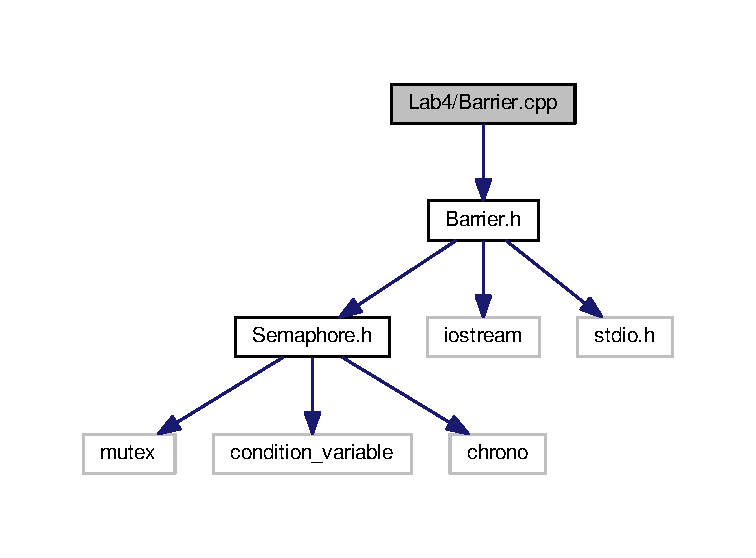
\includegraphics[width=350pt]{_barrier_8cpp__incl}
\end{center}
\end{figure}

\hypertarget{_barrier_8h}{}\section{Lab4/\+Barrier.h File Reference}
\label{_barrier_8h}\index{Lab4/\+Barrier.\+h@{Lab4/\+Barrier.\+h}}
{\ttfamily \#include \char`\"{}Semaphore.\+h\char`\"{}}\\*
{\ttfamily \#include $<$iostream$>$}\\*
{\ttfamily \#include $<$stdio.\+h$>$}\\*
Include dependency graph for Barrier.\+h\+:
\nopagebreak
\begin{figure}[H]
\begin{center}
\leavevmode
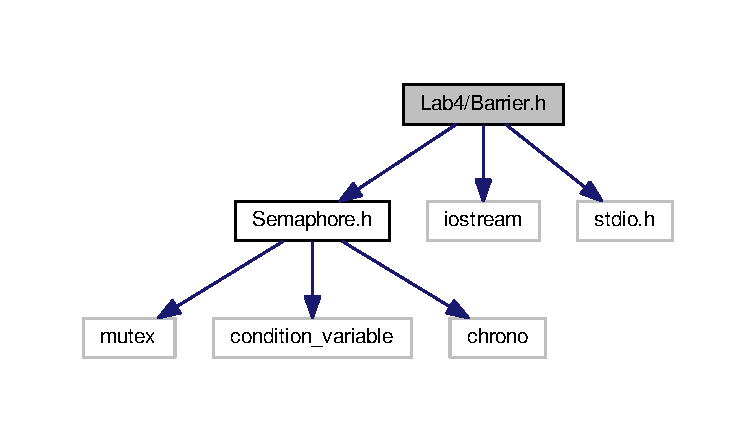
\includegraphics[width=350pt]{_barrier_8h__incl}
\end{center}
\end{figure}
This graph shows which files directly or indirectly include this file\+:
\nopagebreak
\begin{figure}[H]
\begin{center}
\leavevmode
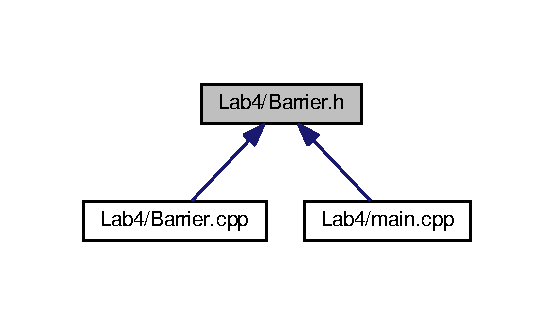
\includegraphics[width=266pt]{_barrier_8h__dep__incl}
\end{center}
\end{figure}
\subsection*{Classes}
\begin{DoxyCompactItemize}
\item 
class \hyperlink{class_barrier}{Barrier}
\begin{DoxyCompactList}\small\item\em An Implementation of a barrier Using Semaphores. \end{DoxyCompactList}\end{DoxyCompactItemize}

\hypertarget{main_8cpp}{}\section{Lab4/main.cpp File Reference}
\label{main_8cpp}\index{Lab4/main.\+cpp@{Lab4/main.\+cpp}}
{\ttfamily \#include \char`\"{}Barrier.\+h\char`\"{}}\\*
{\ttfamily \#include $<$thread$>$}\\*
{\ttfamily \#include $<$vector$>$}\\*
Include dependency graph for main.\+cpp\+:
\nopagebreak
\begin{figure}[H]
\begin{center}
\leavevmode
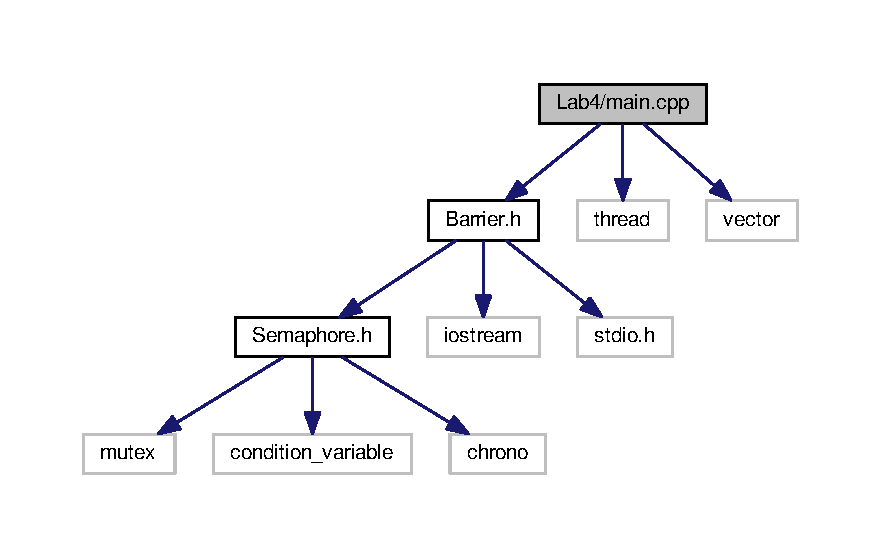
\includegraphics[width=350pt]{main_8cpp__incl}
\end{center}
\end{figure}
\subsection*{Functions}
\begin{DoxyCompactItemize}
\item 
void \hyperlink{main_8cpp_a96ca7eba915789dab4c11886f423c42b}{task} (std\+::shared\+\_\+ptr$<$ \hyperlink{class_barrier}{Barrier} $>$ barrier\+Obj)
\item 
int \hyperlink{main_8cpp_a840291bc02cba5474a4cb46a9b9566fe}{main} (void)
\end{DoxyCompactItemize}


\subsection{Function Documentation}
\index{main.\+cpp@{main.\+cpp}!main@{main}}
\index{main@{main}!main.\+cpp@{main.\+cpp}}
\subsubsection[{\texorpdfstring{main(void)}{main(void)}}]{\setlength{\rightskip}{0pt plus 5cm}int main (
\begin{DoxyParamCaption}
\item[{void}]{}
\end{DoxyParamCaption}
)}\hypertarget{main_8cpp_a840291bc02cba5474a4cb46a9b9566fe}{}\label{main_8cpp_a840291bc02cba5474a4cb46a9b9566fe}
\index{main.\+cpp@{main.\+cpp}!task@{task}}
\index{task@{task}!main.\+cpp@{main.\+cpp}}
\subsubsection[{\texorpdfstring{task(std\+::shared\+\_\+ptr$<$ Barrier $>$ barrier\+Obj)}{task(std::shared_ptr< Barrier > barrierObj)}}]{\setlength{\rightskip}{0pt plus 5cm}void task (
\begin{DoxyParamCaption}
\item[{std\+::shared\+\_\+ptr$<$ {\bf Barrier} $>$}]{barrier\+Obj}
\end{DoxyParamCaption}
)}\hypertarget{main_8cpp_a96ca7eba915789dab4c11886f423c42b}{}\label{main_8cpp_a96ca7eba915789dab4c11886f423c42b}
wait for all thereads to fin before continue 
\hypertarget{_semaphore_8cpp}{}\section{Semaphore.\+cpp File Reference}
\label{_semaphore_8cpp}\index{Semaphore.\+cpp@{Semaphore.\+cpp}}
{\ttfamily \#include \char`\"{}Semaphore.\+h\char`\"{}}\newline
Include dependency graph for Semaphore.\+cpp\+:

\hypertarget{_semaphore_8h}{}\section{Lab4/\+Semaphore.h File Reference}
\label{_semaphore_8h}\index{Lab4/\+Semaphore.\+h@{Lab4/\+Semaphore.\+h}}
{\ttfamily \#include $<$mutex$>$}\\*
{\ttfamily \#include $<$condition\+\_\+variable$>$}\\*
{\ttfamily \#include $<$chrono$>$}\\*
Include dependency graph for Semaphore.\+h\+:
\nopagebreak
\begin{figure}[H]
\begin{center}
\leavevmode
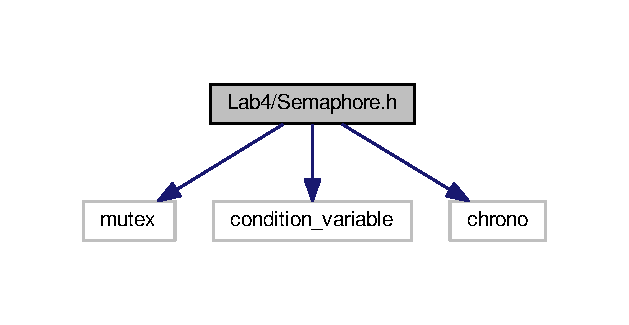
\includegraphics[width=302pt]{_semaphore_8h__incl}
\end{center}
\end{figure}
This graph shows which files directly or indirectly include this file\+:
\nopagebreak
\begin{figure}[H]
\begin{center}
\leavevmode
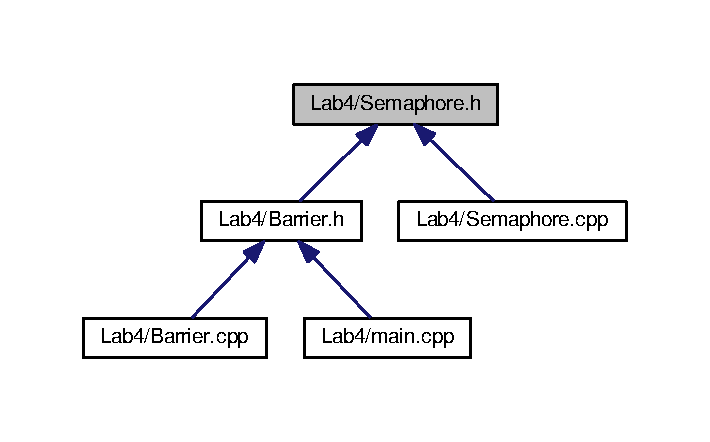
\includegraphics[width=341pt]{_semaphore_8h__dep__incl}
\end{center}
\end{figure}
\subsection*{Classes}
\begin{DoxyCompactItemize}
\item 
class \hyperlink{class_semaphore}{Semaphore}
\begin{DoxyCompactList}\small\item\em A \hyperlink{class_semaphore}{Semaphore} Implementation. \end{DoxyCompactList}\end{DoxyCompactItemize}

%--- End generated contents ---

% Index
\backmatter
\newpage
\phantomsection
\clearemptydoublepage
\addcontentsline{toc}{chapter}{Index}
\printindex

\end{document}
